\documentclass[a0paper, portrait]{tikzposter}
\usepackage[utf8]{inputenc}

%%%%%%%%%%%%%%%%%%%%%%%%
%  table env for tkiz  %
%%%%%%%%%%%%%%%%%%%%%%%%
\newcounter{tablecounter}
\newenvironment{tikztable}[1][]{
  \def \rememberparameter{#1}
  \vspace{10pt}
  \refstepcounter{tablecounter}
  \begin{center}
  }{
    \ifx\rememberparameter\@empty
    \else
    \\[10pt]
    {\small Tab.~\thetablecounter: \rememberparameter}
    \fi
  \end{center}
}
%%%%%%%%%%%%%%%%%%%%%%
 
\title{The Genetic Architecure of Human Aggression}
\author{Robert M. Porsch}
\date{\today}
\institute{Center of Genomic Science}
%\titlegraphic{\includegraphics{1d.jpg}}
 
\usetheme{Simple}
 
\begin{document}
 
\maketitle

\block{Abstract}{ 
Aggression is the delivery of an aversive stimulus from one person to another with intent to cause harm.
Such behavior has potential beneficial and harmful consequences for the aggressor and can be seen to originate in the evolutionary principles of natural selection,
suggesting that genetic factors have a considerable impact on aggressive behavior.

Analysis of the genetic correlations with aggression showed high estimates for risk taking ($r_g=0.44, SE=0.103$), neuroticism ($r_g=0.63, SE=0.083$), and depression ($r_g=0.6741$, $SE=0.0919$).
Interestingly, while a Mendelian randomization approach suggests a causal effect of schizophrenia on both aggression and risk taking, a causal relationship between aggression and depression was not supported.
}

\begin{columns}
  \column{0.5}

    % Aim 
    \block{Aim}{
      \begin{itemize}
        \item Identification of \textbf{genetic loci} associated with impulsive Aggression and Risk Taking
        \item Investigate the \textbf{genetic overlap} between aggression and related phenotypes
        \item Explore \textbf{causal connection} among behavioral phenotypes
      \end{itemize}
    }

    % Methods and Samples
    \block{Methods}{
      \begin{itemize}
        \item Samples from the UK BioBank and publicly available summary statistics were used
        \item Heritability and Genetic Correlations were computed with LD-Score regression
        \item Potential causal pathways between psychiatric disorders and aggression/risk taking were investigated
      \end{itemize}
      \begin{tikztable}[Sample Size and Missingness of UK Biobank]
        \centering
        \input{tables/descriptive_ukb.tex}
      \end{tikztable}
    }

    % Genetic Correlation Matrix
    \block{Genetic Correlations}{
      \begin{tikzfigure}[Genetic Correlations within the UKB]
        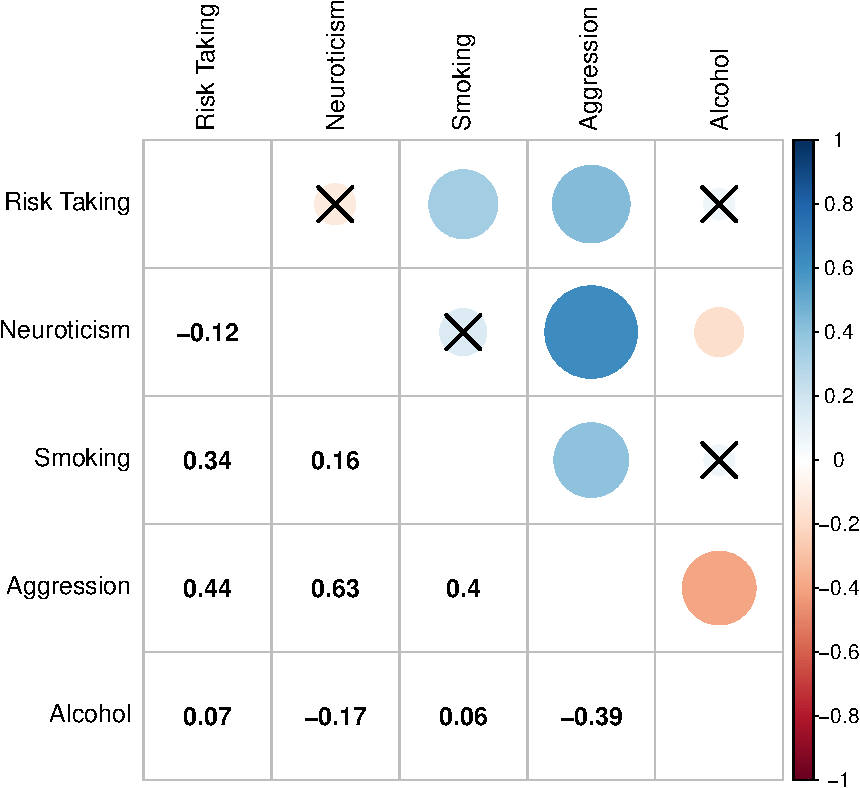
\includegraphics[width=0.65\linewidth]{../ukb_assoc/figure/genetic_corr/gcorr_plot_circle_full_se.pdf}
      \end{tikzfigure}
    }

    % Phenotypic Effects
    \block{Phenotypic Effects}{

      \begin{minipage}{0.49\linewidth}
        \begin{tikzfigure}[Phenotypic Correlations]
          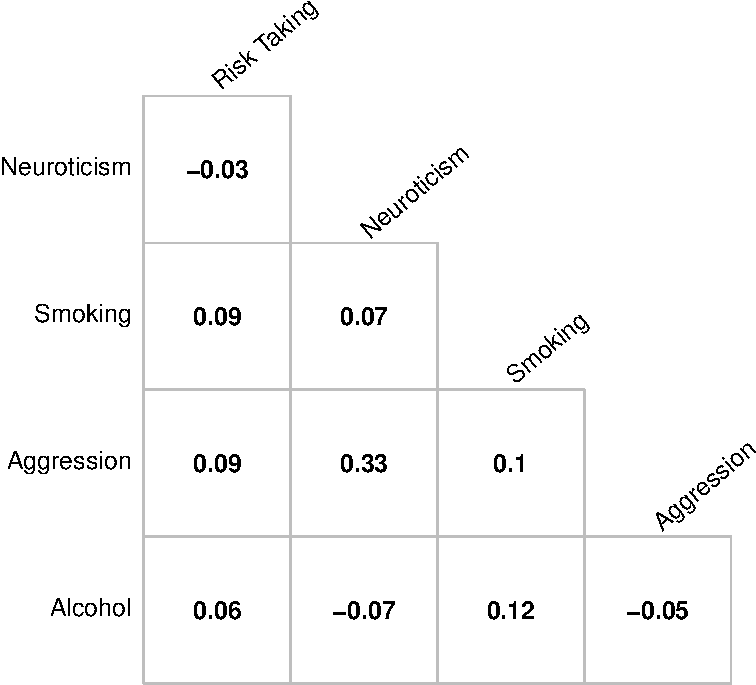
\includegraphics[width=0.99\linewidth]{../ukb_assoc/figure/phenotype/corr_plot_ci.pdf}
        \end{tikzfigure}
      \end{minipage} \hfill
      \begin{minipage}{0.49\linewidth}
        \begin{tikzfigure}[
          Effects of Age (A) and Sex (B) as well as the distrubition of Neuroticisim (C) and drinking behavior (D)
          ]
          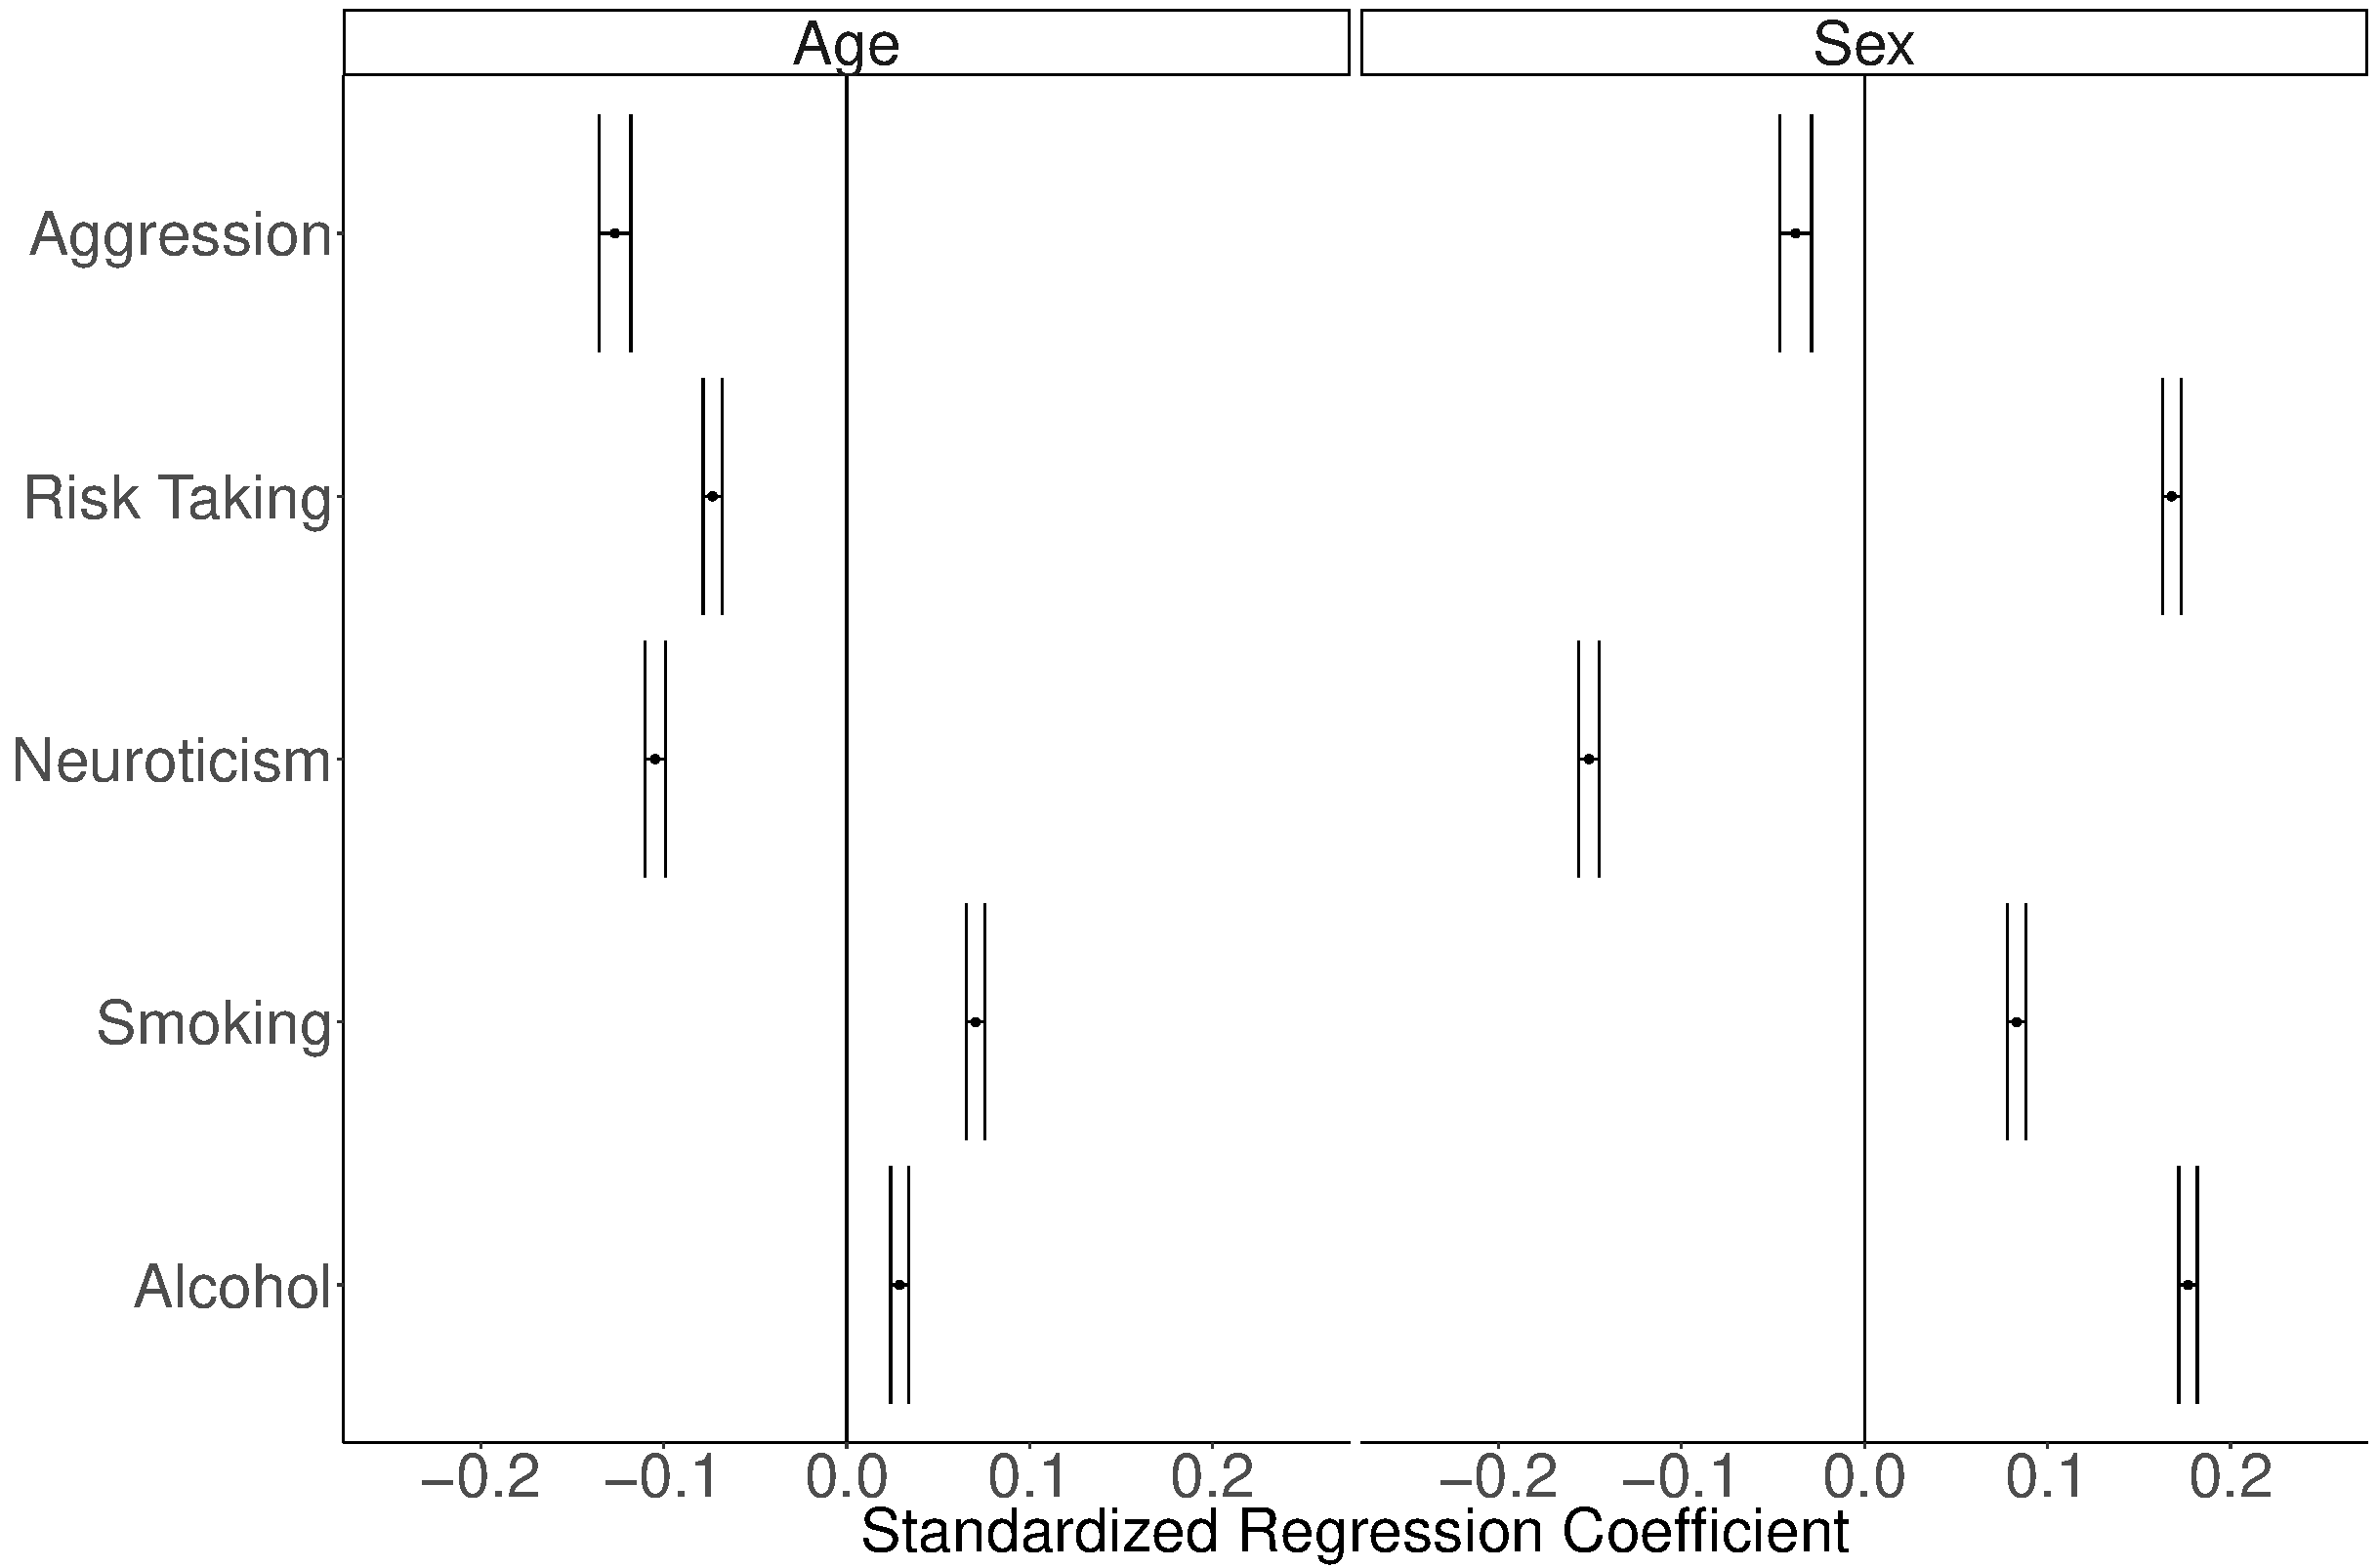
\includegraphics[width=0.99\linewidth]{../ukb_assoc/figure/phenotype/descriptives_plots.pdf}
        \end{tikzfigure}
      \end{minipage}
    }

  \column{0.5}

    % Association Results
    \block{Association Results}{}
\end{columns}

\end{document}
